%this is chapter 3 about Finding benchmarks.

\chapter{FINDING BENCHMARKS}\label{chapter:Finding benchmarks}

%this section is about TPC-H benchmark.
\section{REASEARCHING BENCHMARK.}
\subsection{TPC benchmarks}
\subsubsection{TPC-H}
{\justify
The TPC-H \cite{TPC} is a decision support benchmark. It consists of a suite of business oriented to ad-hoc queries and concurrent data modifications. The queries and the data populating the database have been chosen to have broad industry-wide relevance while maintaning a sufficient degree of ease of implementation. This benchmark illustrates decision support systems that
\begin{itemize}
\item Examine large volumes of data.
\item Execute queries with a high degree of complexity.
\item Give answers to critical business questions.
\end{itemize}
\par }
{\justify
TPC-H evaluates the performance of various decision support systems by the execution of sets of queries against a standard database under controlled conditions. The TPC-H queries:
\begin{itemize}
\item Give answers to real-world business questions.
\item Simulate generated ad-hoc queries (e.g., via a point and click GUI interface);
\item Are far more complex than most OLTP transactions.
\item Include a rich breadth of operators and selectivity constraints;
\item Generate intensive activity on the part of the database server component of the system under test.
\item Are executed against a database complying to specific population and scaling requirements. The relations in this database don't have the correlated data together.
\item Are implemented with constraints derived from staying closely synchronized with an on-line production database. 
\item contains few joins, between 0 to 4 joins each query. For example, 1.sql doesn't have any join in this query, 2.sql contains 3 joins.
\end{itemize}
\par }
\vspace{0.5cm}
%this section is about TPC-DS benchmark.
\subsubsection{TPC-DS}
{\justify
TPC-DS \cite{TPC} is a decision support benchmark that models several generally applicable aspects of a decision support system (DSS), including queries and data maintenance:
\begin{itemize}
\item User queries, which convert operational facts into business intelligence.
\item Data maintenance, which synchronizes the process of managenment analysis with the operational external data source on which it relies.
\end{itemize}
The benchmark provides a representative evaluation of the System Under Test's(SUT) performance as a general purpose decision support system.
\par }
{\justify
TPC-DS illustrates decision support systems that:
\begin{itemize}
\item Examine large volumes of data.
\item Give answers to real-world business questions.
\item Execute queries of various operational requirements and complexities
\item Are characterized by high CPU and IO load
\item Are periodically synchronized with source Online Transaction Porcessing (OLTP) databases through database maintenance functions.
\item Run on "Big Data" solutions, such as RDBMS as well as Hadoop/Spark based systems.
\end{itemize}
\par }
{\justify
There are four broad classes of queries that characterize most decision support queries:
\begin{itemize}
\item Reporting queries: These queries capture the "reporting" nature of a DSS system. They include queries that are executed periodcally to answer well-known, pre-defined questions about the financial and operational health of a business. They tend to be static.
\item Ad hoc queries: These queries capture the dynamic nature of a DSS system in which impromtu queries are constructed to answer immediate and specific business questions.
\item Iterative Online Analytical Processing (OLAP) queries: These queries are used for the exploration and analysis of business data to discover new and meaningful relationships and trends. It is distinguished with Ad hoc queries by a scenario-based user session in which a sequence of queries is submitted.
\item Data mining queries: These queries can be used to predict future trends and behaviors, allowing business to make proactive, knowledge-driven decisions. This class of queries typically consists of joins and large aggregation that return large data result sets for possible extraction.
\end{itemize}
\par }
{\justify
There are joins in each query, especially the queries which are belong to the class of data mining.
\begin{itemize}
\item For example: query 91 contains 6 joins
\end{itemize}
\par }
%TPC-E
\subsubsection{TPC-E}
{\justify
TPC-E \cite{TPC} is an OLTP workload. It is a mixture of read-only and update intensive transactions that simulate the activities found in complex OLTP application environments. The database schema, data population, transactions, and implementation rules have been designed to be broadly representative of modern OLTP systems. It exercises a breadth of system components associated with such environments, which are characterized by:
\begin{itemize}
\item The simultaneous execution of multiple transaction types that span a breadth of complexity.
\item A balanced mixture of disk input/output and processor usage.
\item Transaction integrity.
\item A mixture of uniform and non-uniform data access through primary and secondary keys.
\item Databases consisting of many tables with a wide variety of sizes, attributes, and relationships with realistic content.
\item Contention on data access and update.
\item Moderate system and application execution time.
\end{itemize}
\par }
{\justify
The goal of TPC-E is simulating the OLTP workload of a brokerage firm. The focus of the benchmark is the central database that executes transactions related to the firm's customer accounts. In keeping with the goal of measuring the performance characteristics of the database system, the benchmark does not attempt to measure the complex flow of data between multiple application systems that would exist in a real environment.
\par }
\vspace{0.5cm}
{\justify
There are limitations in this benchmark:
\begin{itemize}
\item Benchmark results are significantly dependent upon workload, specific application requirements, and systems design and implementation. Relative system performance will vary because of those and other factors. Therefore, it should not used as a substitue or specific customer application benchmarking when critical capacity planning and product evaluation decisions are contemplated.
\item There are few joins in each query and the queries totally focus on the transactions.
\end{itemize}
\par }
%this section is about SSB benchmark
\subsection{Star Schema Benchmark}
{\justify
The Star Schema Benchmar (SSB) \cite{SSB} was designed to test star schema optimization to address the issues outlined in TPC-H with the goal of measuring performance of database products and to test a new materialization strategy. It is a simple benchmark that consists of four query flights, four dimensions. The SSB is significantly based on the TPC-H benchmark with improvements that implements a traditional pure star-schema and allows column and table compression.
\par }
\vspace{0.5cm}
{\justify
The SSB is designed to measure performance of database products against a traditional data warehouse scheme. It implements the same logical data in a tradional star schema, whereas TPC-H models the data in pseudo 3NF schema.
\par }
\vspace{0.5cm}
{\justify
Some model queries in SSB benchmar are based on the TPC-H query set, but need to be modified to vary the selectivity. There are the queries that don't have an equal conterpart in TPC-H.
\begin{itemize}
\item Query Flights: Compared to the TPC-H's 22 queries, SSB contains four query flights that each consist of three to four queries that vary selectivity. Each flight consists of a sequence of queries that someone working with data warehouse systems.
\item Caching: One other issue arises in  running the Star Schema Benchmark queries, and that is the caching effect that reduces the number of disk accesses necessary when query Q2 follows query Q1, because of overlap of data accessed between Q1 and Q2. SSB attempts to minimize overlap, however in situations where this cannot be done, SSB will take whatever steps are needed to reduce caching effects of one query on another. 
\end{itemize}
\par }
%this section is about JOB benchmark.
\subsection{JOB benchmark}
{\justify
JOB bechmark \cite{JOB} contains two main components:
\begin{itemize}
\item IMDB Data set: It contains a plethora of information about movies and related facts related actors, directors, production companies. The data is freely available for non-commercial use as text files. Besides, there is an open source, namely imdbpy, to transform the text files into a relational database with 21 tables. As most real-world  data sets, IMDB is full of correlations and non-uniform data distributions, and is therefore much more challenging than most synthetic data sets. Now, The size of this data set is about 20 Gigabytes.
\end{itemize}
\begin{itemize}
\item JOB queries: They are based on the IMDB data set and is constructed as analytical SQL queries. They focus on join ordering, which argualy is the most important query optimization problem. They were designed to have between 3 and 16 joins, with an average of 8 joins per query. For example, Query 13d, which finds the ratings and release dates for all movies produced by US companies, contains 11 joins.
\end{itemize}
{
Figure 5 is the typical query grapth of JOB workload. In this graph, The solid edges in the graph represent key/foreign key edges (1 : n) with the arrow head pointing to the primary key side. Dotted edges represent foreign key/foreign key joins (n : m), which appear due to transitive join predicates.
\par }
{
\begin{figure}[H]
\centering
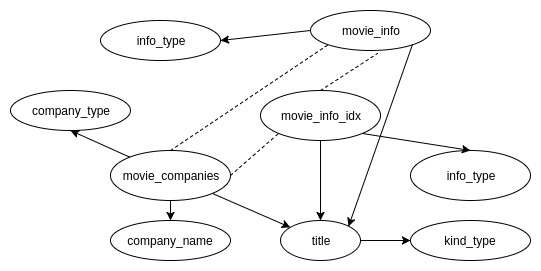
\includegraphics[width=1.0\textwidth]{query_graph_JOB.jpg}
\caption{Typical query graph of JOB workload.}
\end{figure}
}
{
For cardinality estimators the queries are challenging due to the significant number of joins and the correlations contained in the dataset. However, The queries did not try to “trick” the query optimizer, e.g., by picking attributes with extreme correlations. Also, they intentionally did not include more complex join predicates like inequalities or non-surrogate-key predicates, because cardinality estimation for this workload is already quite challenging.
\par }
}
\section{CONCLUSION}
{\justify
Although TPC-H, TPC-E, TPC-DS or the Star Schema Benchmark (SSB) have proven their value for evaluating query engines, I argue that they are not good bechmark for the cardinality estimation component of query optimizers. The reason is that in order to easily be able to scale the benchmark data, the data generators are using the very same simplifying assumptions (uniformity, independence, principle of inclusion) which are the reasons leading to the limitaions of cardinality estimator of PostgresSQL and that query optimizers make. Real-world data sets, in contrast, are full of correlations and non-uniform data distributions, which makes cardinality estimation much harder. Therefore, I don't use these benchmarks for benchmarking the cardinality estimation component of PostgreSQL's query optimizer.
\par }
\vspace{0.5cm}
{\justify
Besides, JOB benchmark solved the limitations of the benchmarks above. Their queries contain many joins and their data set are full of correlations and non-uniform data distributions, which makes cardinality estimator of PostgreSQL encounter many hardships. So it is very suitable to be used for benchmarking cardinality estimation component of PostgreSQL's optimizer.
\par }
\vspace{0.5cm}

